\documentclass{beamer}

\usepackage{amsmath}
\usepackage{subcaption}


\title{Beamer}
\author{Simon Willimann}
\institute{University of Zurich}
\date{04.11.2021}

\begin{document}

\frame{\titlepage}


\begin{frame}
\frametitle{Equation}
\framesubtitle{Subtitle1}
	\begin{equation*}
		\begin{aligned}
		SS{n} = & \ SSI_n*0.4 + \frac{B_n}{20}*0.2 + \frac{R_n}{20}*0.2 + \frac{S_n}{8}*0.2
		\end{aligned}
	\end{equation*} 

\end{frame}


\begin{frame}
\frametitle{Theorem}
\framesubtitle{Subtitle2}

\begin{theorem}[Pythagorean theorem]
	\label{pythagorean}
	On a right triangle with shorter sides x and y, the long side z always equals
	\[ z^2 = x^2 + y^2 \]
\end{theorem}

\end{frame}



\begin{frame}
\frametitle{Figure}
\framesubtitle{Not sure what's meant by "2 panels", though}

	\begin{figure}[h]
	\centering
	\makebox[\textwidth][c]{  
		\begin{subfigure}[b]{0.5\linewidth}
   		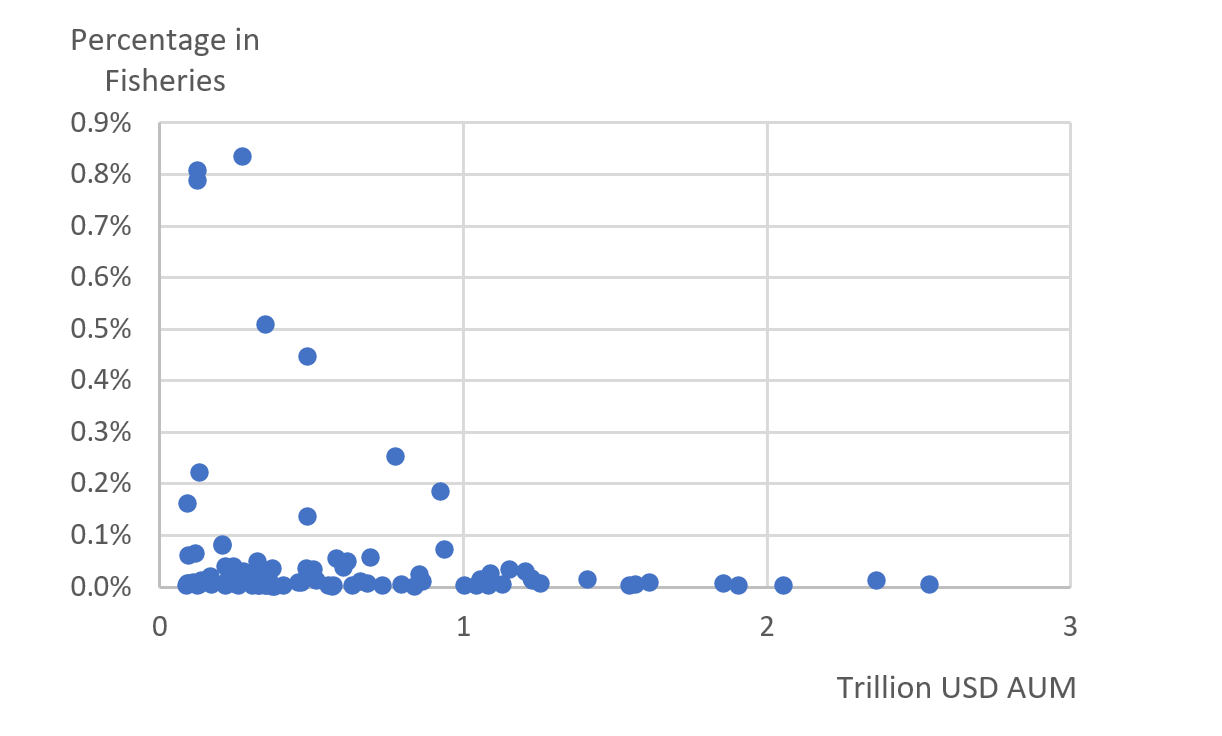
\includegraphics[width=\linewidth]{AUMP.png}
   		\caption{Exposure to Fisheries in Percentage}
 		\end{subfigure}
 		\begin{subfigure}[b]{0.5\linewidth}
		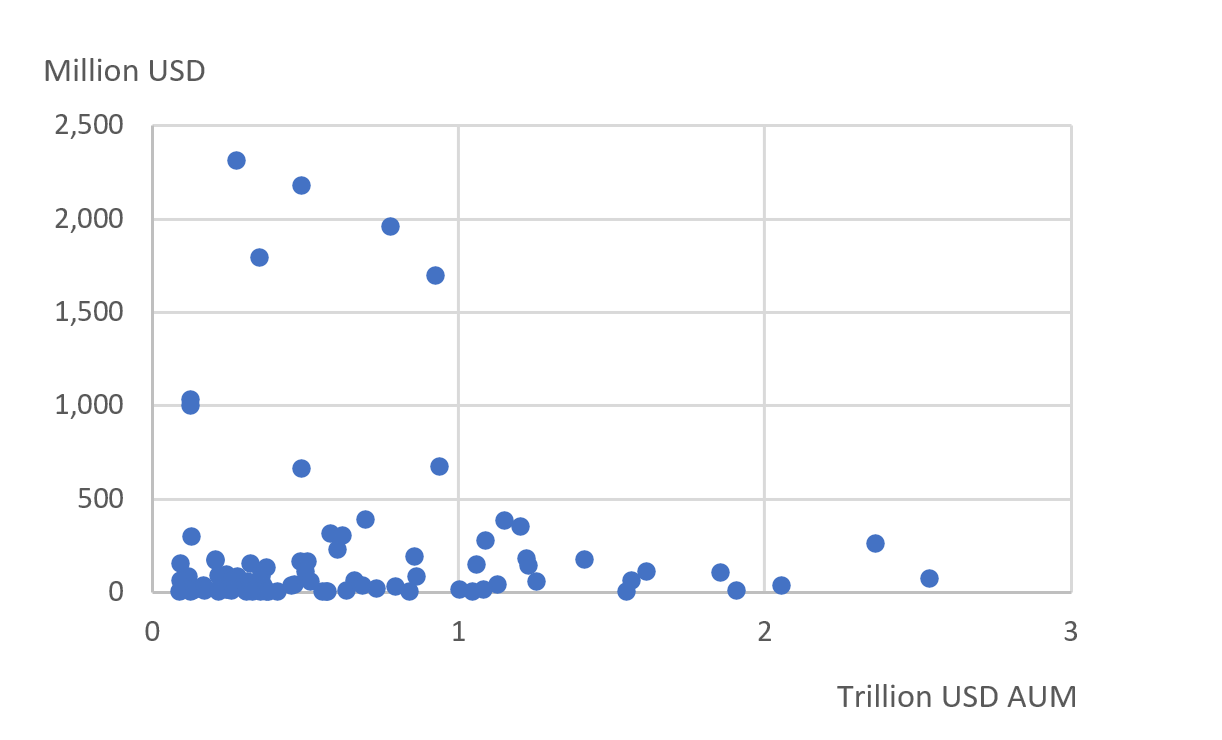
\includegraphics[width=\linewidth]{AUMUSD.png}
		\caption{Exposure to Fisheries in USD}
 		\end{subfigure}}
 		\caption{Exposure of Asset Managers to to Fisheries}
	\end{figure}


\end{frame}



\end{document}